\section{Space as Resource}
Space plays a vital role in advancing science, technology, and the broader progress of humanity. Through the exploration of space, scientists gain unique insights into the origins of the universe, the behavior of physical laws under extreme conditions, and the potential for life elsewhere in the universe. Along with scientific descoveries, technological developments driven by space research often find critical applications on Earth. From satellite communications to microwaves, space technology improves everyday life and drives innovation across industries. Beyond tangible benefits, space exploration fosters curiosity, unity, and ambition, encouraging humanity to transcend borders and collaborate on solving challenges that face us collectively. As we expand our presence outside Earth, space becomes not only a frontier of discovery but also a catalyst for technological and social progress on a global scale.

\section{Space as a Manufacturing Environment}
In-space manufacturing is currently experiencing a surge in interest due to the decreasing cost per kilogram of putting payloads into orbit. With the expectation that Starship will soon reduce the price from around \$1000/kg to \$150/kg~\cite{nextbigfuture2024spacex}, there will be a plethora of new opportunities available to those that can successfully leverage this exotic environment. Microgravity, high vacuum and abundant solar energy are all inherent to space, while remaining very expensive to achieve on Earth. Therefore, products that can utilise these during the manufacturing process would be more cost competitive or of a higher quality than those made on the ground.

In many state-of-the-art materials, fabrication under microgravity results in bigger crystal growth and a more homogenous structure~\cite{issnll_mccg}. This is hugely beneficial for superconducting applications as they are constrained by the inability to sustain high currents, a limitation caused by the presence of grain boundaries~\cite{hilgenkamp2002grain}. Superconductors are, therefore, a perfect candidate for in-space manufacturing and higher quality crystals could unlock new terrestrial applications.

In the longer term, an industrial base in low earth orbit would also have significant implications for the future of space. A harsh constraint on all current missions is the violent launch conditions that the spacecraft's structure must withstand before it reachs orbit. Manufacturing or assembling key components in space would circumvent this, increasing mission flexibility and reliability. At present, solar sail technology is limited by payload fairing dimensions and must fold down to fit within these. If the frames were manufactured in orbit, it would massively decrease mission complexity, enabling new propulsion platforms.

\newpage
\section{Additive Manufacturing in Space CLEAN}
Additive manufacturing, also known as 3D printing, is a transformative technology that enables the layer-by-layer construction of complex structures from stock material. This approach is particularly well suited to space manufacturing due to its significantly lower material waste, high design flexibility, and the ease of transporting feedstock like filament or powder. Prefabricated components like I-beams or plates can impose strict constraints on launch vehicle payload dimensions.!! Whereas raw materials for additive manufacturing are compact, lightweight, and adaptable to a wide range of mission needs.

For structural components of any space mission, the requirements to be compact enough to fit into the payload fairing and strong enough to withstand the launch vibrations sacrifice [efficiency and reliability wantt o get across big optimisation problem]. If these parts are manufactured once they are in orbit, the designs can be tailored to the orbital manoeuvre loads alone, increasing mission flexibility. !!

Additionally!!, the crucial benefit of additive manufacturing is its ability to repair and modify existing components. This capability is especially valuable in space, where repairs can!! be challenging and costly. By enabling on-demand production of spare parts or modifications to existing systems, additive manufacturing enhances the resilience and longevity of space missions, reducing the need for extensive inventories of spare parts and minimizing the risk of mission failure due to component obsolescence or damage. !!

\section{Previous Work and Motivation CLEAN}
The current line of research exploring Cold Spray Additive Manufacturing (CSAM) in space started with an analysis of different additive manufacturing methods and how they were impacted by properties of the space environment such as microgravity, thermal constraints and elevated exposure to radiation. Despite the requirement to bring a propellant gas to orbit with the manufacturing facility, the combination of not requiring post processing, flexibility of being able to spray onto unprepared metal surfaces and high deposition rate made CSAM an attractive candidate for further research~\cite{malagowski2019amspace}.

This analysis was later followed up with COSMOS, a technical demonstration of CSAM under vacuum conditions. The demonstration was a success and samples of the aluminium deposit were produced and analysed. After the analysis, it was found that the porosity of the deposit was higher than expected. This is thought to be because the mass flow rate of the powder was too high, meaning the particles were not accelerated to a high enough velocity and so!! did not deform as expected. In addition to this, the design of the powder hopper was not suitable for a microgravity environment. These two issues provide the key motivation to this project.

\newpage

\section{Objectives}
As mentioned, the previous powder hopper design, seen in \autoref{fig:current-feed-system-exploded-diagram}, was not suitable for microgravity applications. It resembles a typical fluidized powder bed used in the chemical engineering industry, seen in \autoref{fig:fluidized-bed-diagram}, where the gas flows from bottom to top and, given a high enough flow rate, entrains the particles into the flow.
\begin{figure}[htbp]
    \centering

    \begin{minipage}{0.3\textwidth}
        \centering
        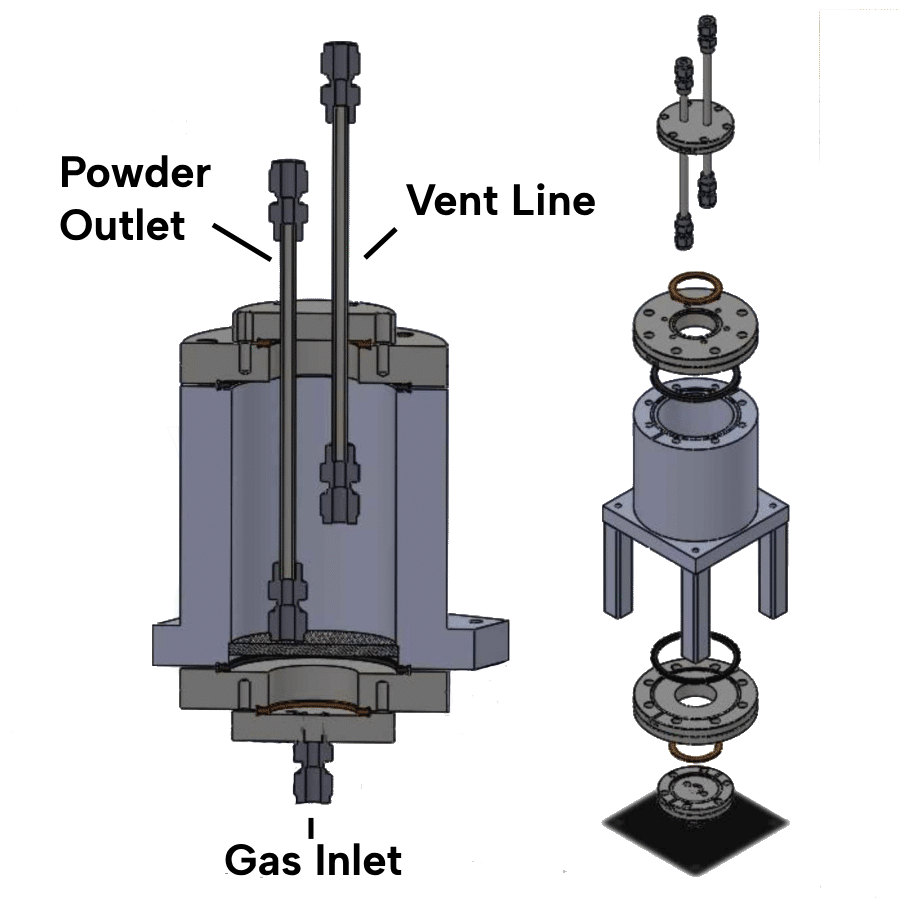
\includegraphics[width=\textwidth]{../report_assets/COSMOS_DIAGRAM.png}
        \caption{Current feed system diagram.}\label{fig:current-feed-system-exploded-diagram}
    \end{minipage}
    \hfill
    \begin{minipage}{0.3\textwidth}
        \centering
        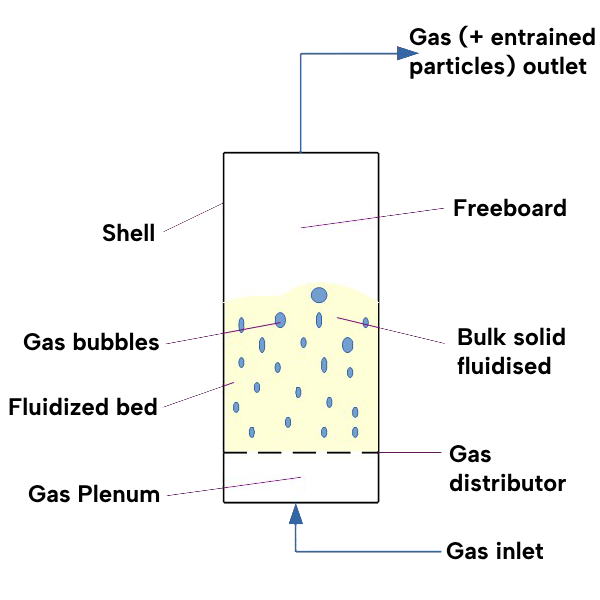
\includegraphics[width=\textwidth]{../report_assets/Fluidized_Bed_polished.png}
        \caption{Simplified fluidized powder bed diagram.}\label{fig:fluidized-bed-diagram}
    \end{minipage}
    \hfill
    \begin{minipage}{0.3\textwidth}
        \centering
        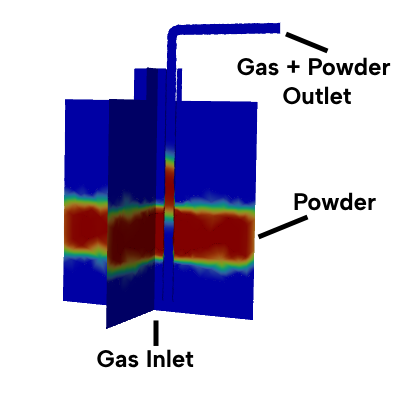
\includegraphics[width=\textwidth]{../report_assets/configuration_that_demands_pms.png}
        \caption{Fluent simulation in microgravity.}\label{fig:current-feed-system-fluent}
    \end{minipage}

\end{figure}

While it was more than suitable to facilitate the testing of the CSAM system, it would be prone to disruption due to the powder moving away from the outlet. This is because the powder, that sat on top of the mesh in the experiments, is not constrained to this location by anything but gravity. Therefore, if the tank were to recieve a sloshing perturbance, the powder would float off the mesh and away from the outlet. To verify this idea and demonstrate that the powder would not be dispersed throughout the whole tank due to turbulent mixing, a fluent simulation was conducted, seen in \autoref{fig:current-feed-system-fluent}. Even after 10s of simulation time the system reached steady state with no mixing or powder dispersion, necesitating a redesign.

Building on all this previous work, the primary objectives of the project were to develop and characterise a tank capable of producing a constant and controllable mass flow rate as well as operating reliably under microgravity. The tank must:
\begin{itemize}
    \item Constrain the powder to the outlet of the system,
    \item Design for controlability of the mass flow rate,
    \item Prioritise low mass and high reliability.
\end{itemize}
And to characterise this system, the relationship between pressure into the system and mass flow rate out must be defined through:
\begin{itemize}
    \item Analysing the relationship between piston velocity and mass flow rate,
    \item Analysing the relationship between pressure differentials across the piston face and the corresponding velocity,
    \item Determine key factors in piston geometry that affect the pressure differential.
\end{itemize}